\chapter{Introduction}

Computational and signal processing tasks can be performed by digital circuits, since they are robust and can be realized by small and simple structures to obtain complex, fast and accurate systems. As the time passes the speed and density of digital integrated circuits have increased, but the physical world has remained the same, which means that the data converters are still needed to be able to communicate with it by utilizing digital signal processing (DSP). One thing to note is that digital circuits in the modern technology offers fast transistors biased at low voltage, which introduces drawbacks in the analog design such as the short-channel effects and larger leakage currents.  

Analog-to-digital (ADC) converters are an important part of microcontrollers and system-on-chip (SoC) products. More applications demand higher resolution and slower converters, for example for applications such as battery management and sensor measurement. This is driven by the desire to measure very small input signals, for which a $\Delta\Sigma$ ADC is very suitable. Figure \ref{comp_asdc} exhibit  the trade-off between accuracy and speed for various ADC structures. The fastest one with lowest obtainable resolution is flash ADC. With a conversion speed of 1GHz it can only achieve a resolution up to 8 bits. The reason being the area grows proportional with $2^M$ (Where M is the number of bits). The folding and SAR ADCs mange to give better resolution than the flash ADC, but at the cost of slower conversion speed. These can be used on applications which require medium speed and medium resolution. Pipeline ADC is good to use to achieve resolution up to 14 bits with a high conversion speed from 1MHz to 100MHz. When high resolution is required, the integrating ADC is a good alternative, but it requires $2^M$ clock periods to convert a single sample. Hence, it is a good choice for applications with high resolution and very low frequency demand.The ADCs discussed are Nyquist-rate converter, and as seen they cannot not provide good accuracy with high speed.  Oversampling converters like $\Delta\Sigma$ converters on the other hand are well suited, with high resolution acquisition and low power consumption. They are also widely used ADC architecture, as they relax the requirements of the analog building blocks by the use of oversampling and noise-shaping.

\begin{figure}[H]
\centering
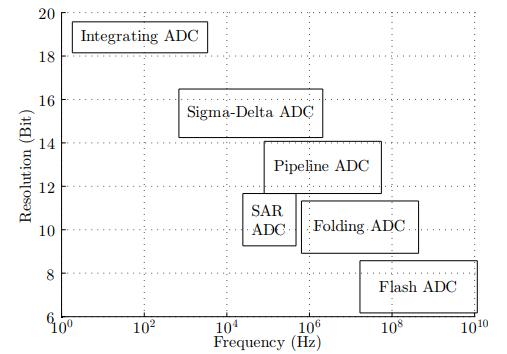
\includegraphics[scale = 0.7]{images/compare_adc.png}
\caption{Bandwidth and resolution specifications of different ADC architecture}
\label{comp_asdc}
\end{figure}

However the design of $\Delta\Sigma$ is not a easy task, as it relies on analog design techniques as well as advanced filtering and signal  processing techniques. To find a good architecture depends on proper modelling of the behaviour of the converter. 

\section{Thesis Contribution}
This thesis aims at showing the design and implementation of a $\Delta\Sigma$ modulator based on the feasibility study done in Autumn. The main objective is to achieve approximately 16 bits resolution and manage to sample it at 10MHz. The modulator was designed using 180nm complementary-metal-oxide-semiconductor (CMOS) process technology with 1.8V of supply voltage. The modulator implemented is a third order discrete time modulator which uses three low pass filters, latched comparator acting as a 1-bit quantizer and a 1-bit feedback digital-to-analog (DAC) to obtain the desired resolution. 

Figure \ref{intro_design_flow} depict the design flow of the $\Delta\Sigma$ modulator. It can be seen that a higher level define specification for a lower level. A bottom-up approach was used to verify the system i.e. starting with verifying from transistor-level and working up to system-level. The work can be divided into three stages, as described below.  



\begin{figure}[H]
\centering
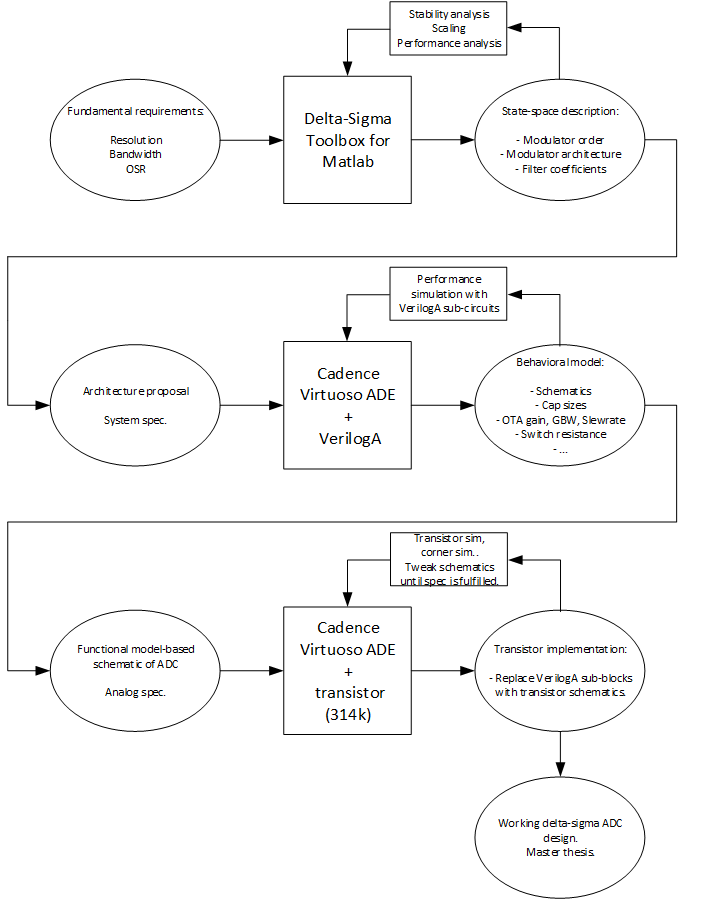
\includegraphics[scale = 0.6]{images/design_slow.png}
\caption{Design flow of the $\Delta\Sigma$ modulator}
\label{intro_design_flow}
\end{figure}

\textbf{The model was first synthesized using Richard. Schreier’s $\Delta\Sigma$ toolbox in MatLab\cite{tool}} based on the fundamental requirements, such as resolution, bandwidth and OSR. The results from the toolbox were used to derive a state description based on the modulator order, filter coefficients, number of bits of the quantizer and loop topology. Stability and performance analysis were performed in order to maintain the modulator's integrity.

\textbf{VerilogA was used to implement} the analog blocks from the architectural performance. Behavioral model was done by Cadence Virtuoso ADE to derive the specifications of the analog blocks such that the fabrication process variations do not affect the system performance.

\textbf{Finally the VerilogA models} were replaced by transistor schematics. These schematics were verified according to the specifications found in behavioural modeling using nominal and process, supply voltage and temperature variations (PVT simulations) using Spectre. 

\section{Thesis outline}

\textbf{Chapter 2 - Background theory}: The fundamentals of $\Delta\Sigma$, concept of oversampling . noise-shaping and switched-capacitor circuits are presented. Additionally the theory behind the $g_m/I_D$ methodology is also presented. 

\textbf{Chapter 3 - Proposed architecture}: The decision of the architecture based on loop filter order, topologies, time-domain, number of quantizer bit and operational transconductance amplifier (OTA) is also discussed. 

\textbf{Chapter 4 - Specifications of the design}:
The results obtained in the feasibility study is summarized and discussed here. They were used as specifications to implement the analog blocks in transistor level. 

\textbf{Chapter 5 - Circuit design}: It contains the complete design methodology adopted to the successful implementation of the modulator. It also presents the analysis and the design of the analog blocks used, such as: switches, two phase clock generator, OTAs and comparator.    

\textbf{Chapter 6 - Results}: Here the results and discussion of all the blocks designed and implemented is presented, where the results is presented by both nominal and PVT simulations. The nominal and PVT simulations of the whole modulator is given as a final results for the thesis. 

\textbf{Chapter 7 - Conclusion} : A summary and conclusion of the work is presented. some suggestion regarding the future work that can sought is also presented. 